\documentclass[../Moduli_Spaces_of_Riemann_Surfaces.tex]{subfiles}

\begin{document}
    \section{Overview and Main Results}
    Complex analysis in the plane is an extremely rich theory with many important features, but is topologically not very interesting. On the other hand, general topological spaces are too badly-behaved for any reasonable analysis to be done, so a middle-ground must be found. To leverage the desired properties of $\C$, we restrict the class of topological spaces of study to those with a local neighborhood around every point that looks like a deformed patch of $\C$, but whose global behaviour can be quite different. The choice in which a topological space is made to look locally like $\C$ is called a \textit{complex structure}, and, in general, there are many such choices. A topological space $X$, equipped with a particular choice of complex structure, is called a \textit{Riemann surface}.\\\ \\
    As a motivating example, take the torus $T^2$. Around every point $p\in T^2$, we can find a small enough neighborhood $U$ of $p$ that deforms reversibly onto an open subset of $\C$. The figure below shows two ways of doing so.
    \begin{center}
        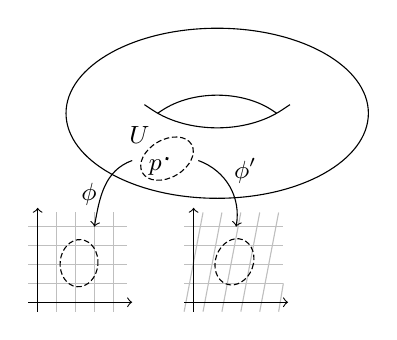
\begin{tikzpicture}[scale=1.2]
            \draw (0,0) ellipse (1.6 and 0.9);
            \begin{scope}[scale=0.7]
                \draw[rounded corners = 28pt] (-1.1,0.13) -- (0,-0.6) -- (1.1,0.13);
                \draw[rounded corners = 24pt] (-0.9,0) -- (0,0.6) -- (0.9,0);
            \end{scope}
            \begin{scope}[rotate=30, xshift=-0.7cm, yshift=-0.15cm]
                \fill (0,0) circle (0.008in) node[xshift=-0.15cm, yshift=-0.12cm]{\small$p$};
                \fill (0,0) circle (0) node[xshift=-0.35cm, yshift=0.3cm]{\small$U$};
                \draw[dash pattern={on 2pt off 1pt}] (0,0) ellipse (0.3 and 0.2);
            \end{scope}
            \begin{scope}[xshift=-1.9cm, yshift=-2cm]
                \draw[lightgray, step=0.2] (-0.1,-0.1) grid (0.95,0.95);
                \draw[->] (-0.1,0) -- (1,0);
                \draw[->] (0,-0.1) -- (0,1);
                \begin{scope}[rotate=-5]
                    \draw[dash pattern={on 2pt off 1pt}] (0.4,0.45) ellipse (0.2 and 0.25);
                \end{scope}
            \end{scope}
            \begin{scope}[xshift=-0.25cm, yshift=-2cm]
                \draw[lightgray] (-0.1,0.2) -- (0.95,0.2);
                \draw[lightgray] (-0.1,0.4) -- (0.95,0.4);
                \draw[lightgray] (-0.1,0.6) -- (0.95,0.6);
                \draw[lightgray] (-0.1,0.8) -- (0.95,0.8);
                \draw[lightgray] (-0.1,-0.1) -- (0.1,0.95);
                \draw[lightgray] (0.1,-0.1) -- (0.3,0.95);
                \draw[lightgray] (0.3,-0.1) -- (0.5,0.95);
                \draw[lightgray] (0.5,-0.1) -- (0.7,0.95);
                \draw[lightgray] (0.7,-0.1) -- (0.9,0.95);
                \draw[lightgray] (0.9,-0.1) -- (0.95,0.2);
                \draw[->] (-0.1,0) -- (1,0);
                \draw[->] (0,-0.1) -- (0,1);
                \begin{scope}[rotate=-20]
                    \draw[dash pattern={on 2pt off 1pt}] (0.26,0.55) ellipse (0.2 and 0.25);
                \end{scope}
            \end{scope}
            \draw[->] (-0.9,-0.5) to[out=200, in=80] node[xshift=-0.2cm, yshift=-0.1cm]{\small$\phi$} (-1.3,-1.2);
            \draw[->] (-0.2,-0.5) to[out=-20, in=80] node[xshift=0.2cm, yshift=0.2cm]{\small$\phi'$} (0.2,-1.2);
        \end{tikzpicture}
    \end{center}
    Using $\phi$ to `pull' the coordinate lines back to $U$, we see that the angles that they make is different from the angles made by using $\phi'$ instead. The rigidity of holomorphic maps from complex analysis suggests that those coordinates ought to be different, and indeed they are. Thus we see that the same topological space, $T^2$, can be equipped with many different complex structures, making them different \textit{complex tori}.\\\ \\
    In general, we call the set of all complex structures on $X$ the \textit{moduli space\footnote{This paper is only concerned with the underlying set of points, without regard to any geometric structure. This turns out to be interesting enough in its own right, but the reader should be aware that the study of geometric structures on the moduli space is vast. We refer the interested reader to \cite{i&t}, \cite{farb}, and \cite{hubbard}.} of $X$}, and the main goal of this paper is to compute it for the sphere $S^2$ and the torus $T^2$. The results, proven in Theorem \ref{MS:thm:simply-connect_compact_biholomorphic_Riemann_sphere} and Corollary \ref{MS:cor:moduli_space_torus} respectively, are as follows.
    \begin{itemize}
        \item Surprisingly, the moduli space of $S^2$ is a point. In other words, the sphere admits a unique complex structure. This fact, which is part of the \textit{Uniformization Theorem}, is one of the starting points in the theory of compact Riemann surfaces, which we will spend the majority of this paper discussing.
            \vspace{-0.05in}
        \item The fact that $T^2$ can be constructed topologically as a quotient $\C/\Gamma$ by an integer lattice $\Gamma$ gives us a relatively straightforward proof that the moduli space of $T^2$ is $\H/\!\PSL{2}{\Z}$. Here, $\H\subset\C$ is the upper-half plane of $\C$ and $\PSL{2}{\Z}\coloneqq\SL_2\!\l(\Z\r)\!/\!\l\{\pm I\r\}$ is the \textit{modular group}, which acts on $\H$ via Möbius transformations. We show that all complex tori can be written as $X_\tau\coloneqq\C/\!\l(\Z\oplus\tau\Z\r)$ for some $\tau\in\H$, and two tori $X_\tau$ and $X_{\tau'}$ are biholomorphic iff $\tau$ and $\tau'$ lie in the same orbit of the action.
    \end{itemize}
\end{document}
